% Cours 4 - Problèmes hyperboliques et méthode des caractéristiques

\documentclass[
mode=present,    % "present" or "print" or "handout"
paper=a4paper,   % "screen" or "a4paper"
orient=landscape,
display=slides,   % "slides" or "slidesnotes" or "notes"
size=10pt,
style=romain   % default, simple, fyma, ciment, horatio, paintings, jefka, ...
]{powerdot}

\usepackage{mypdotstyle}

\graphicspath{ {cours04/fig/} }

\pdsetup{
cf={MATH0471 -- Cours 4},
lf={ULg, Liège, Belgium},
trans=Replace,  % Split, Blinds, Box, Wipe, Dissolve, Glitter, Replace
  }

\begin{document}

    % reduction of the space before and after equations
    % (must be after "\begin{document}")
    \setlength{\belowdisplayskip}{2pt}
    \setlength{\belowdisplayshortskip}{2pt}
    \setlength{\abovedisplayskip}{2pt}
    \setlength{\abovedisplayshortskip}{2pt}

\title{\vspace{-5mm}
         {\sl\small MATH0471 -- Projet de calcul scientifique multiphysique} \\
        \vspace{5mm}
        \Large Problèmes hyperboliques et méthode des caractéristiques\\
        \vspace{5mm}
}
\author{R. Boman \& C. Geuzaine}
\date{\today}
\maketitle

%=======================================================================
% TABLE DES MATIERES
%=======================================================================

\begin{slide}[toc=,bm=]{Table des matières}
\tableofcontents[content=sections] % sections, all
\end{slide}
%=======================================================================


%=======================================================================
\section[toc=Lien math0024]{Lien avec le cours d'EDP (math0024)}
%=======================================================================

%-----------------------------------------------------------------------
\begin{slide}[toc=Ellipticité]{Notion d'ellipticité}
%-----------------------------------------------------------------------

Rappel du cours d'EDP (lecture-1 part C):

\vspace{\stretch{1}}

\noindent\fbox{\parbox{\linewidth-2\fboxrule-2\fboxsep}{ %-----------------------------------------------------------

Une EDP linéaire à coefficients constant d'ordre $k$ est \textbf{elliptique} si:
\begin{itemize}
\item les coefficients des dérivées partielles d'ordre $k$ ne sont pas nuls,
\item il n'existe pas un changement de variables pour lequel un de ces coefficients s'annule.
\end{itemize}
}} %-----------------------------------------------------------------------------------------------------------------

\vspace{\stretch{1}}

Cette notion permet, en pratique:
\begin{itemize}
\item de résoudre certains types d'EDP,
\item d'appliquer le bon nombre de conditions aux limites sur la frontière du domaine étudié,
\item comprendre la physique derrière un système d'équations complexes,
\item choisir une méthode numérique appropriée.
\end{itemize}

\end{slide}


%-----------------------------------------------------------------------
\begin{slide}[toc=Equ. Poisson]{Notion d'ellipticité}
%-----------------------------------------------------------------------

\emph{Exemple 1:} Equation de Poisson

\begin{equation*}
\frac{\partial^2 u}{\partial^2 x} + \frac{\partial^2 u}{\partial^2 y} =  f
\end{equation*}
est \textbf{elliptique} car le changement de variable

\begin{equation*}
     \begin{bmatrix}
        x \\
        y
    \end{bmatrix}
    \mapsto
    \begin{bmatrix}
        \tilde{x} \\
        \tilde{y}
    \end{bmatrix}
    =
    \begin{bmatrix}
        A_{\tilde{x}x} & A_{\tilde{x}y} \\
        A_{\tilde{y}x} & A_{\tilde{y}y}
    \end{bmatrix}
    \begin{bmatrix}
        x \\
        y
    \end{bmatrix}
\end{equation*}
donne une équation du type:
\begin{equation*}
\underbrace{(A_{\tilde{x}x}^2 + A_{\tilde{x}y}^2)}_{\neq 0}
\frac{\partial^2 u}{\partial^2 x} +
\underbrace{(A_{\tilde{y}x}^2 + A_{\tilde{y}y}^2)}_{\neq 0}
\frac{\partial^2 u}{\partial^2 y} + ... =  f
\end{equation*}

Les coefficients ne peuvent pas s'annuler si le changement de variable n'est pas singulier ($\det [A]\neq 0$).

\end{slide}


%-----------------------------------------------------------------------
\begin{slide}[toc=Equ. chaleur]{Notion d'ellipticité}
%-----------------------------------------------------------------------

\emph{Exemple 2:} Equation de la chaleur

\begin{equation*}
\frac{\partial u}{\partial t} - \frac{\partial^2 u}{\partial^2 x} =  f
\end{equation*}
n'est \textbf{pas elliptique}.

\bigskip

En effet, sans même changer de variables, il n'y a pas de terme en $\displaystyle\frac{\partial^2 u}{\partial^2 t}$

\bigskip
En chaque point $(x,t)$, on peut définir une \textbf{ligne caractéristique} qui est la ligne normale à la direction selon laquelle l'équation n'est pas du second ordre.

    \centerline{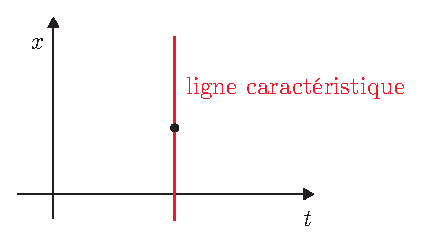
\includegraphics[width=0.45\textwidth]{parabolic.eps} }

\end{slide}


%-----------------------------------------------------------------------
\begin{slide}[toc=Equ. ondes]{Notion d'ellipticité}
%-----------------------------------------------------------------------

\emph{Exemple 3:} Equation d'ondes

\begin{equation*}
\frac{\partial^2 u}{\partial^2 t} -c^2\, \frac{\partial^2 u}{\partial^2 x} =  f
\end{equation*}

\bigskip

n'est \textbf{pas elliptique} car le changement de variable
\begin{equation*}
     \begin{bmatrix}
        x \\
        t
    \end{bmatrix}
    \mapsto
    \begin{bmatrix}
        \tilde{x} \\
        \tilde{t}
    \end{bmatrix}
    =
    \begin{bmatrix}
        A_{\tilde{x}x} & A_{\tilde{x}t} \\
        A_{\tilde{t}x} & A_{\tilde{t}t}
    \end{bmatrix}
    \begin{bmatrix}
        x \\
        t
    \end{bmatrix}
\end{equation*}
donne une équation du type:

\begin{equation*}
\underbrace{(A_{\tilde{x}t}^2 -c^2 A_{\tilde{x}x}^2)}_{=0 \text{ si } A_{\tilde{x}t} = \pm c A_{\tilde{x}x} }
\frac{\partial^2 u}{\partial^2 \tilde{x}} +
\underbrace{(A_{\tilde{t}t}^2 -c^2 A_{\tilde{t}x}^2)}_{=0 \text{ si } A_{\tilde{t}t} = \pm c A_{\tilde{t}x}}
\frac{\partial^2 u}{\partial^2 \tilde{t}} + ... =  f
\end{equation*}.

Choisir $A_{\tilde{x}t} = \pm c A_{\tilde{x}x}$ correspond à un changement de variable du type $\tilde{x} = A_{\tilde{x}x} \, (x\pm c\,t)$. Similairement au cas précédent, les lignes $(x\pm c\,t)=C^{\text{te}}$, c'est-à-dire celles où $\tilde{x}$ est constant, sont appelées \textbf{lignes caractéristiques}.

\end{slide}


%-----------------------------------------------------------------------
\begin{slide}[toc=]{Notion d'ellipticité}
%-----------------------------------------------------------------------

Choisir $A_{\tilde{t}t} = \pm c A_{\tilde{t}x}$ correspond à un changement de variable du type $\tilde{t} = A_{\tilde{t}x} \, (x\pm c\,t)$. Les lignes $(x\pm c\,t)=C^{\text{te}}$, c'est-à-dire celles où $\tilde{t}$ est constant, sont appelées lignes caractéristiques.

\bigskip

    \centerline{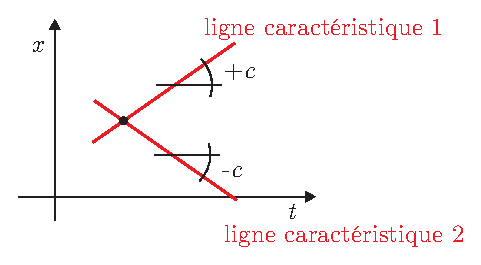
\includegraphics[width=0.55\textwidth]{hyperbolic.eps} }

\vspace{\stretch{1}}

La suite de ce cours explique l'utilité pratique de ces lignes caratéristiques.

\vspace{\stretch{1}}

\end{slide}



%=======================================================================
\section[toc=Carac. 2D - 1equ.]{Méthode des caractéristiques pour 1 équation à 2 variables indépendantes}
%=======================================================================


%-----------------------------------------------------------------------
\begin{slide}[toc=Courbes caractéristiques]{Courbes caractéristiques}
%-----------------------------------------------------------------------

Soit
\begin{equation*}
a\, \frac{\partial u}{\partial t} + b\, \frac{\partial u}{\partial x} = c
\end{equation*}

où $a, b, c$ peuvent être constants ou dépendre de $x, t, u$ mais pas des dérivées de $u$, ce qui revient à dire que
l'équation quasi-linéaire.

Écrivons l'équation sous la forme:
\begin{equation*}
\sqrt{a^2+b^2} \left( \underbrace{\frac{a}{\sqrt{a^2+b^2}}}_{\cos\theta}\, \frac{\partial u}{\partial t} + \underbrace{\frac{b}{\sqrt{a^2+b^2}}}_{\sin\theta}\, \frac{\partial u}{\partial x} \right) = c
\end{equation*}

\begin{minipage}[l]{\textwidth/2}
    \centerline{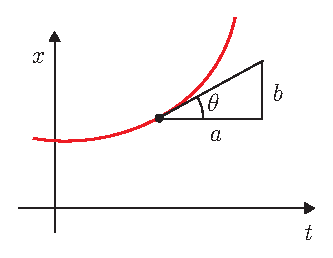
\includegraphics[width=0.7\textwidth]{intro1d.eps} }
\end{minipage}
\begin{minipage}[l]{\textwidth/2-1cm}
    \begin{equation*}
        \tan\theta = \boxed{ \frac{dx}{dt} = \frac{b}{a} }
    \end{equation*}

    \bigskip

    Les courbes définies par cette EDO sont appelées \textbf{courbes caractéristiques}.
\end{minipage}

\end{slide}



%-----------------------------------------------------------------------
\begin{slide}[toc=Equ. caractéristique]{Equation caractéristique - inv. de Riemann}
%-----------------------------------------------------------------------

L'équation s'écrit:
\begin{equation*}
    \cos\theta \frac{\partial u}{\partial t} + \sin\theta \frac{\partial u}{\partial x} = \frac{c}{\sqrt{a^2+b^2}}
\end{equation*}

\bigskip

Le membre de droite est la dérivée de $u$ selon l'abscisse curviligne (notée $s$) de la ligne caractéristique. On a donc:
\begin{equation*}
    \boxed{ \frac{d u}{ds} = \frac{c}{\sqrt{a^2+b^2}} }
\end{equation*}

L'EDP initiale s'exprime comme une EDO le long d'une ligne caractéristique. On l'appelle \textbf{équation caractéristique}.

\bigskip

\emph{Remarque:} si $c=0$, on a
\begin{equation*}
    \frac{d u}{ds} = 0 \qquad \Rightarrow \quad u=C^{\text{te}}
\end{equation*}
La solution $u$ est constante le long d'un ligne caractéristique donnée.
$u$ est alors un \textbf{invariant de Riemann}.



\end{slide}



%-----------------------------------------------------------------------
\begin{slide}[toc=Résumé]{Résumé de la méthode}
%-----------------------------------------------------------------------

\emph{Résumé:}
\begin{equation*}
a(u,x,t)\, \frac{\partial u}{\partial t} + b(u,x,t)\, \frac{\partial u}{\partial x} = c
\end{equation*}

\begin{enumerate}
\item En chaque point on peut évaluer $b/a$ qui est la pente locale de la courbe caractéristique passant par ce point. Si c'est possible (si $a$ et $b$ sont constants p. expl.), on peut intégrer l'équation $\frac{dx}{dt}=b/a$ pour obtenir la forme des lignes caractéristiques.
\item L'EDP devient une EDO, le long de ces lignes:
    \begin{equation*}
    \frac{d u}{ds} = \frac{c}{\sqrt{a^2+b^2}}
    \end{equation*}
\item La solution de l'EDP est obtenue en intégrant cette équation.
\item Si $c=0$, on a un invariant de Riemann ($u=C^{\text{te}}$).
\end{enumerate}

\end{slide}


%-----------------------------------------------------------------------
\begin{slide}[toc=Exemple]{Exemple simple}
%-----------------------------------------------------------------------

\emph{Exemple simple:}

\begin{equation*}
2 \frac{\partial u}{\partial t} + \frac{\partial u}{\partial x} = 0
\end{equation*}

\bigskip

Equation des lignes caractéristiques:
\begin{equation*}
\frac{dx}{dt} = \frac{b}{a} = \frac{1}{2}
\end{equation*}
\begin{equation*}
\Rightarrow x(t) = \int \frac{b}{a} \, dx = \frac{1}{2} \, t + C
\end{equation*}

Il s'agit d'un réseau de droites de pente 1/2.

\bigskip

L'équation s'écrit le long de ces lignes (équation caractéristique):
    \begin{equation*}
    \frac{d u}{ds} = 0 \qquad \Rightarrow \quad u=C^{\text{te}}
    \end{equation*}


\end{slide}



%-----------------------------------------------------------------------
\begin{slide}[toc=]{Exemple simple}
%-----------------------------------------------------------------------

La solution de l'équation un un point donné du domaine de calcul dépend donc de la solution qu'on va imposer sur les bords du domaine.

\bigskip

    \centerline{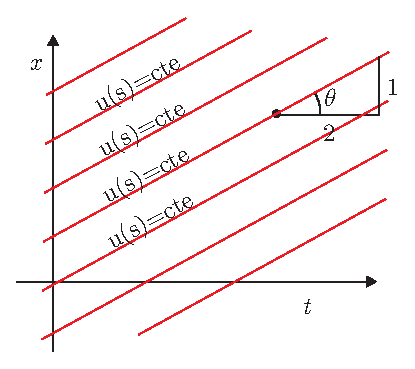
\includegraphics[width=0.45\textwidth]{carac1d.eps} }

\bigskip

Comme on a un invariant de Riemann, la solution se ``propage'' le long des lignes caractéristiques


\end{slide}


%-----------------------------------------------------------------------
\begin{slide}[toc=Cauchy pur]{Problème de Cauchy pur}
%-----------------------------------------------------------------------

\textbf{Problème de Cauchy pur}: on résout l'EDP sur un domaine spatial infini à partir d'une valeur initiale de $u$.

\bigskip

Exemple de problème de Cauchy pur où $a$ et $b$ dépendent uniquement de $u$
\begin{equation*}
\frac{\partial u}{\partial t} + u(x)\, \frac{\partial u}{\partial x} = 0
\end{equation*}
\bigskip

    \centerline{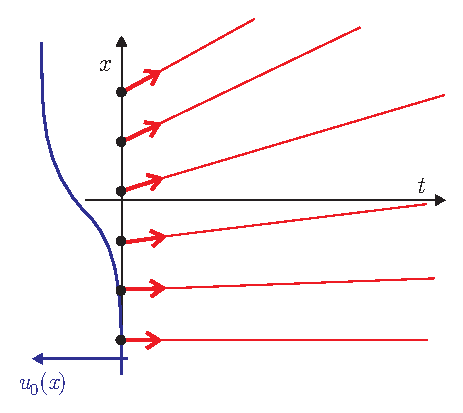
\includegraphics[width=0.45\textwidth]{cauchy1d.eps} }

\end{slide}


%-----------------------------------------------------------------------
\begin{slide}[toc=]{Problème de Cauchy pur}
%-----------------------------------------------------------------------

Remarque: domaine d'influence des conditions initiales

\bigskip

    \centerline{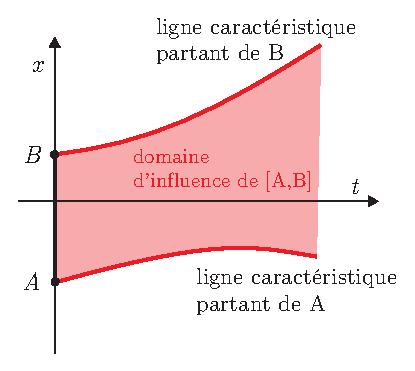
\includegraphics[width=0.45\textwidth]{dominfl1d.eps} }

Modifier les conditions initiales sur un segment $[A,B]$ modifiera la solution uniquement dans une zone du plan $(t,x)$ délimitée par les caractéristiques partant de $A$ et $B$. On appelle cette zone le \textbf{domaine d'influence} de $[A,B]$

\end{slide}



%-----------------------------------------------------------------------
\begin{slide}[toc=Cauchy mixte / CL]{Problème de Cauchy mixte - Choix des C.L.}
%-----------------------------------------------------------------------

Problème de Cauchy mixte. Le domaine spatial n'est plus infini.

\bigskip

    \centerline{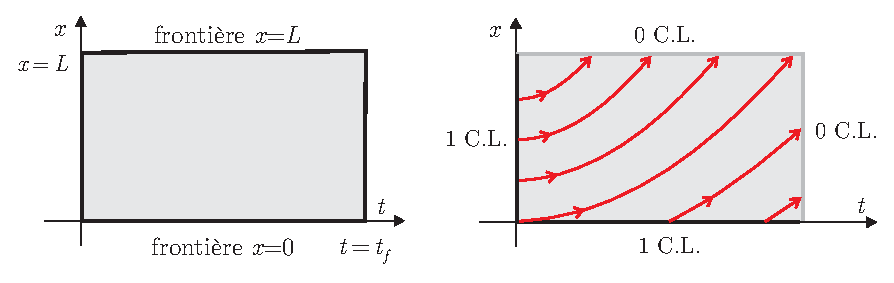
\includegraphics[width=0.9\textwidth]{mixte1d.eps} }

Le nombre de conditions aux limites à appliquer (1 ou 0) dépend de la valeur de la pente des lignes caractéristiques évaluée au niveau des frontières du domaine.

\bigskip

Remarque:
\begin{itemize}
\item Cette pente peut dépendre de la solution (lorsque $a$ et/ou $b$ dépendent de $u$)!
\end{itemize}
\end{slide}


%-----------------------------------------------------------------------
\begin{slide}[toc=]{Problème de Cauchy mixte - Choix des C.L.}
%-----------------------------------------------------------------------

Généralement, même dans des cas très simples, plusieurs possibilités sont envisageables.

\bigskip

    \centerline{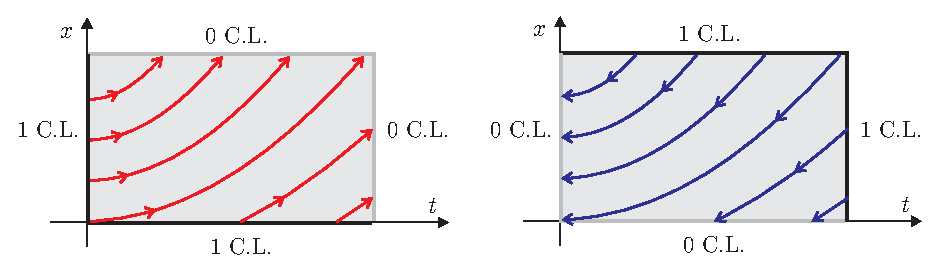
\includegraphics[width=0.9\textwidth]{clbis1d.eps} }

C'est alors la physique qui permet de décider~: dans ce cas-ci ``remonter le temps'', comme le suggère les C.L. de droite n'a pas de sens.

\bigskip

Les conclusions pourraient être différentes si les deux variables indépendantes étaient des variables spatiales $(t,x)\rightarrow(x,y)$.
\end{slide}


%-----------------------------------------------------------------------
\begin{slide}[toc=]{Problème de Cauchy mixte - Choix des C.L.}
%-----------------------------------------------------------------------

Exemple dans le plan $(x,y)$:

    \centerline{\includegraphics[width=0.45\textwidth]{domqcq1d.eps} }

\bigskip

Pour ce type de problème, les zones où on applique 1 condition et celles où on n'applique rien sont séparées par les points de tangence du réseau de lignes caractéristiques au domaine spatial étudié.

\end{slide}


%=======================================================================
\section[toc=Carac. 2D - 2equ.]{Méthode des caractéristiques pour 2 équations à 2 variables indépendantes}
%=======================================================================


%-----------------------------------------------------------------------
\begin{slide}[toc=Systèmes]{Extension à plusieurs équations}
%-----------------------------------------------------------------------

Ce qui vient d'être présenté peut être étendu aux équations d'ordre plus élevé (ou aux systèmes - c'est équivalent).

\bigskip

Par exemple:
\begin{equation*}
\frac{\partial^2 u}{\partial t^2} -\varepsilon\, a^2\, \frac{\partial^2 u}{\partial x^2} = b \qquad (\varepsilon=\pm 1)
\end{equation*}
avec, en toute généralité, $a=a(\partial_t u, \partial_x u, u, t , x)$ et $b=b(\partial_t u, \partial_x u, u, t , x)$.

\bigskip\bigskip

Cette équation se transforme aisément en un système du premier ordre:
        \begin{equation*}
            \left\{
            \begin{aligned}
                & \frac{\partial q}{\partial t} -\varepsilon\, a^2\, \frac{\partial p}{\partial x} = b     \\
                & \frac{\partial p}{\partial t} -\frac{\partial q}{\partial x} = 0
            \end{aligned}
            \right.
        \end{equation*}
où on a posé $q=\partial_t u$ et $p=\partial_x u$.

\end{slide}


%-----------------------------------------------------------------------
\begin{slide}[toc=]{Extension à plusieurs équations}
%-----------------------------------------------------------------------

Comme précédemment, on recherche une direction selon laquelle les dérivées partielles se transforment en dérivées par rapport à une seule variable qui serait l'abscisse curviligne d'une courbe.

\bigskip

Pour y arriver, on effectue une combinaison linéaire des équations:
        \begin{equation*}
            \left\{
            \begin{aligned}
                & \left( \frac{\partial q}{\partial t} -\varepsilon\, a^2\, \frac{\partial p}{\partial x} = b \right)  &\qquad \times\sigma   \\
                & \left( \frac{\partial p}{\partial t} -\frac{\partial q}{\partial x} = 0 \right)  &\qquad \times\lambda
            \end{aligned}
            \right.
        \end{equation*}
et on rassemble les termes en $p$ et en $q$:
        \begin{equation*}
\underbrace{\left[ \sigma \frac{\partial}{\partial t} - \lambda \frac{\partial}{\partial x}  \right]}_{\displaystyle l_1=\frac{d x}{d t}=-\frac{\lambda}{\sigma}}\, q
\quad + \quad
\underbrace{\left[ \lambda \frac{\partial}{\partial t} -\varepsilon\, a^2 \sigma \frac{\partial}{\partial x}  \right]}_{\displaystyle l_2=\frac{d x}{d t}=-\frac{\varepsilon\, a^2 \sigma}{\lambda}}\, p = \sigma\, b
        \end{equation*}

Si $l_1=l_2$, les pentes coïncident et on peut transformer les dérivées partielles en dérivées selon $s$.

\end{slide}


%-----------------------------------------------------------------------
\begin{slide}[toc=]{Extension à plusieurs équations}
%-----------------------------------------------------------------------

Exprimons la condition $l_1=l_2$:
        \begin{equation*}
l = -\frac{\lambda}{\sigma} = -\frac{\varepsilon\, a^2 \sigma}{\lambda}
        \end{equation*}
On peut choisir $\sigma$ et $\lambda$ pour vérifier cette relation. Les 2 égalités ci-dessous fournissent le système:
        \begin{equation*}
            \left\{
            \begin{aligned}
                & \sigma\,l+\lambda = 0   \\
                & \lambda\,l +\varepsilon\, a^2 \sigma = 0
            \end{aligned}
            \right.
        \end{equation*}
sous forme matricielle:
        \begin{equation*}
            \begin{bmatrix}
                 l   & 1   \\
                \varepsilon\, a^2 & l
            \end{bmatrix}
            \begin{bmatrix}
                 \sigma   \\
                \lambda
            \end{bmatrix}
            =
            \begin{bmatrix}
                 0  \\
                0
            \end{bmatrix}
        \end{equation*}
Ce système a une solution non triviale si
        \begin{equation*}
            \det \begin{bmatrix}
                 l   & 1   \\
                \varepsilon\, a^2 & l
            \end{bmatrix}
            =0
            \qquad
            \Rightarrow \quad
            l^2-\varepsilon\, a^2 = 0
        \end{equation*}
\end{slide}


%-----------------------------------------------------------------------
\begin{slide}[toc=Cas elliptique]{Cas elliptique}
%-----------------------------------------------------------------------

\emph{Si $\varepsilon=-1$:}

\bigskip

L'équation a 2 solutions complexes: $\boxed{ l_{1,2}=\pm i\,a }$

\bigskip

Les pentes recherchées sont complexes. Il n'est donc pas possible de tracer des lignes caractéristiques. Le système est \textbf{elliptique}.



\end{slide}



%-----------------------------------------------------------------------
\begin{slide}[toc=Cas hyperbolique]{Cas hyperbolique}
%-----------------------------------------------------------------------

\emph{Si $\varepsilon=+1$:}

\bigskip

L'équation a 2 solutions réelles: $\boxed{ l_{1,2}=\pm a }$

\bigskip

On a donc trouvé deux pentes caractéristiques ($l_1$ et $l_2$). Ces pentes définissent deux réseaux de lignes caractéristiques dont la forme ($x=x_1(t)$ et $x=x_2(t)$) peut être déduite en intégrant les équations:

\bigskip

\begin{minipage}[l]{\textwidth/2}
    \centerline{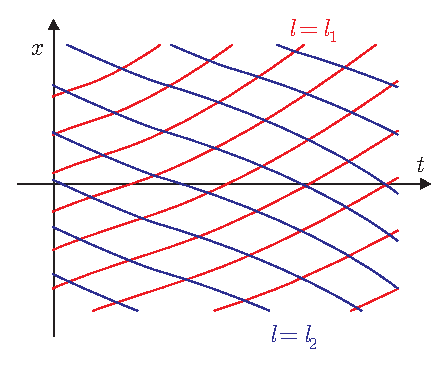
\includegraphics[width=0.8\textwidth]{carac2.eps} }
\end{minipage}
\begin{minipage}[l]{\textwidth/2-1cm}
        \begin{equation*}
            \left\{
            \begin{aligned}
                & \frac{d x_1}{d t} = +a(p,q,u,x,t)   \\
                & \frac{d x_2}{d t} = -a(p,q,u,x,t)
            \end{aligned}
            \right.
        \end{equation*}
\end{minipage}

Le système est \textbf{hyperbolique}.

\end{slide}




%-----------------------------------------------------------------------
\begin{slide}[toc=Equ. caractéristiques]{Equations caractéristiques}
%-----------------------------------------------------------------------

Que devient le système d'équations selon ces lignes?

Il suffit de chercher les valeurs de $\sigma$ et $\lambda$ qui donnent $l=\pm a$

\begin{equation*}
    \left\{
    \begin{aligned}
        & \sigma\,l+\lambda = 0   \\
        & \lambda\,l +\varepsilon\, a^2 \sigma = 0
    \end{aligned}
    \right.
    \quad \Rightarrow
        \left\{
    \begin{aligned}
        & \pm \sigma\,a+\lambda = 0   \\
        & \pm \lambda\,a +\varepsilon\, a^2 \sigma = 0
    \end{aligned}
    \right.
    \quad \Rightarrow \lambda = \mp \sigma\, a
\end{equation*}

et remplacer dans la combinaison linéaire initiale.

\bigskip

Transformons tout d'abord cette combinaison linéaire:
        \begin{equation*}
\left[ \sigma \frac{\partial}{\partial t} - \lambda \frac{\partial}{\partial x}  \right]\, q
 +
\left[ \lambda \frac{\partial}{\partial t} -\varepsilon\, a^2 \sigma \frac{\partial}{\partial x}  \right]\, p = \sigma\, b
        \end{equation*}

        \begin{equation*}
\Rightarrow \cancel{\sigma} \left[ \frac{\partial}{\partial t} + l \frac{\partial}{\partial x}  \right]\, q
\mp \cancel{\sigma}\, a \left[ \frac{\partial}{\partial t} + l \frac{\partial}{\partial x}  \right]\, p = \cancel{\sigma}\, b
        \end{equation*}

\end{slide}


%-----------------------------------------------------------------------
\begin{slide}[toc=]{Equations caractéristiques}
%-----------------------------------------------------------------------

Réécrivons les termes en $p$ et $q$ sous forme de dérivées dans la direction des lignes caractéristiques:

    \centerline{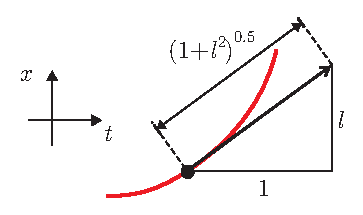
\includegraphics[width=0.35\textwidth]{pente.eps} }

        \begin{equation*}
\underbrace{\left[ \frac{\partial}{\partial t} + l \frac{\partial}{\partial x}  \right]}_{=\displaystyle \sqrt{1+l^2}\frac{d}{ds}}\, q
 \mp a \underbrace{\left[ \frac{\partial}{\partial t} + l \frac{\partial}{\partial x}  \right]}_{=\displaystyle \sqrt{1+l^2}\frac{d}{ds}}\, p = b
        \end{equation*}

\bigskip

        \begin{equation*}
\boxed{ \frac{dq}{ds}
\mp a \frac{dp}{ds} = \frac{b}{\sqrt{1+l^2}} } \qquad\text{(équations caractéristiques)}
        \end{equation*}


\end{slide}




%-----------------------------------------------------------------------
\begin{slide}[toc=Inv. de Riemann]{Invariants de Riemann}
%-----------------------------------------------------------------------

En d'autres termes, si $\varepsilon=1$, l'EDP du second ordre initiale peut être résolue en résolvant simultanément 2 EDOs le long de 2 réseaux de lignes caractéristiques:

        \begin{equation*}
\frac{dq}{ds} - a \frac{dp}{ds} = \frac{b}{\sqrt{1+a^2}}  \qquad\text{le long des courbes de pente } l_1=+a
        \end{equation*}

        \begin{equation*}
\frac{dq}{ds} + a \frac{dp}{ds} = \frac{b}{\sqrt{1+a^2}}  \qquad\text{le long des courbes de pente } l_2=-a
        \end{equation*}

\bigskip

Cas particulier important: $b=0$ et $a=C^{\text{te}}$
        \begin{equation*}
\frac{d}{ds} (q\mp a\,p)  = 0  \qquad\text{le long des courbes de pente } l=\pm a
        \end{equation*}
c'est-à-dire
        \begin{equation*}
q\mp a\,p = C^{\text{te}}  \qquad\text{le long des courbes de pente } l=\pm a
        \end{equation*}

On dit que le système possède 2 \textbf{invariants de Riemann}.

\end{slide}




%-----------------------------------------------------------------------
\begin{slide}[toc=]{Invariants de Riemann}
%-----------------------------------------------------------------------

Si l'EDP possède 2 invariants de Riemann, la résolution du problème initial revient à résoudre en chaque point $(x,t)$ un \textbf{système algébrique d'équations}!

    \centerline{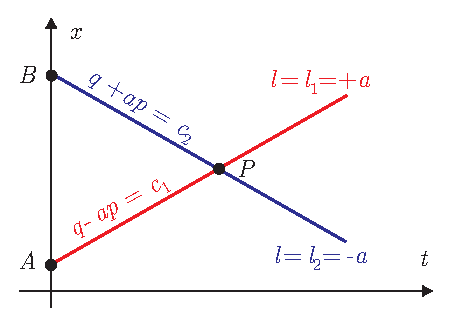
\includegraphics[width=0.4\textwidth]{riemann.eps} }

\begin{equation*}
    \left\{
    \begin{aligned}
        & (q-a\,p)_P = (q-a\,p)_A   \\
        & (q+a\,p)_P = (q+a\,p)_B
    \end{aligned}
    \right.
    \Rightarrow
    \left\{
    \begin{aligned}
        & q_P = \frac{1}{2}(q_B+q_A)+\frac{a}{2}(p_B+p_A)   \\
        & p_P = \frac{1}{2}(p_B-p_A)+\frac{1}{2a}(q_B-q_A)
    \end{aligned}
    \right.
\end{equation*}

La solution en $P$ ne dépend que des valeurs en $A$ et en $B$.

\end{slide}



%-----------------------------------------------------------------------
\begin{slide}[toc=Cauchy pur]{Problème de Cauchy pur}
%-----------------------------------------------------------------------

L'étude des pentes caractéristiques permet de choisir le nombre correct de conditions aux limites à imposer pour obtenir un problème bien posé.

\bigskip

Cas d'un problème de Cauchy pur ($x\in]-\infty, +\infty[, t\ge0$) et de 2 invariants de Riemann:

\bigskip

\begin{minipage}[l]{\textwidth/2}
    \centerline{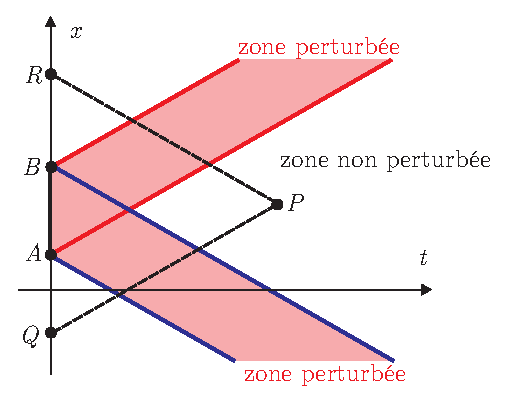
\includegraphics[width=\textwidth]{perturiemann.eps} }
\end{minipage}
\begin{minipage}[l]{\textwidth/2-1cm}
Les conditions aux limites imposées en $[A,B]$ influence la zone mise en évidence délimitée par les caractéristiques partant de $A$ et $B$.
\bigskip

Par contre, la zone où se situe $P$ ne subit aucune influence de $[A,B]$.
\end{minipage}

\end{slide}


%-----------------------------------------------------------------------
\begin{slide}[toc=]{Problème de Cauchy pur}
%-----------------------------------------------------------------------

Si, par contre, il n'existe pas d'invariant de Riemann, la solution en un point est obtenue par intégration des deux équations caractéristiques (EDO) le long des lignes qui aboutissent à ce point.

\bigskip

\begin{minipage}[l]{0.4\textwidth}
    \centerline{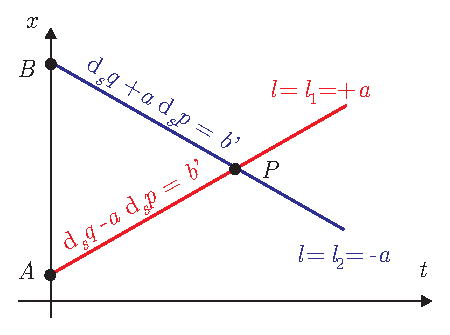
\includegraphics[width=\textwidth]{pasriemann.eps} }
\end{minipage}
\begin{minipage}[l]{0.55\textwidth}
La solution en $P$ est solution de:

\begin{equation*}
    \left\{
    \begin{aligned}
        & \frac{dq}{ds} - a \frac{dp}{ds} = \frac{b}{\sqrt{1+a^2}} \text{ (sur rouge)}  \\
        & \frac{dq}{ds} + a \frac{dp}{ds} = \frac{b}{\sqrt{1+a^2}} \text{ (sur bleue)}
    \end{aligned}
    \right.
\end{equation*}
\end{minipage}

\bigskip

La solution en $P$ dépend de tous les points qui le précèdent sur les deux caractéristiques.

\end{slide}



%-----------------------------------------------------------------------
\begin{slide}[toc=]{Problème de Cauchy pur}
%-----------------------------------------------------------------------

Sans invariant de Riemann, une modification des valeurs de la solution sur la frontière a une influence plus grande.

    \centerline{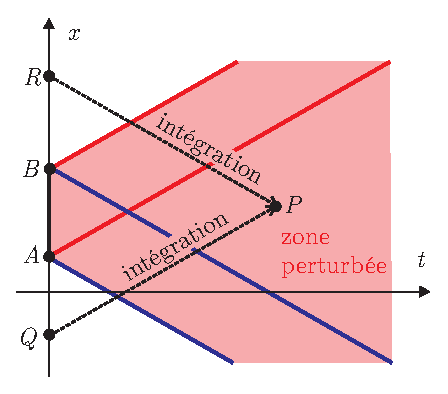
\includegraphics[width=0.4\textwidth]{pertupasriemann.eps} }

\bigskip

Toute la zone comprise entre les lignes caractéristiques partant de $A$ et $B$ est influencée par les valeurs de la solution sur $[A,B]$.

\end{slide}



%-----------------------------------------------------------------------
\begin{slide}[toc=Cauchy mixte / CL]{Problème de Cauchy mixte - Choix des C.L.}
%-----------------------------------------------------------------------

Problème de Cauchy mixte ($x\in[0, L], t\ge0$). Le raisonnement est identique si on a ou non des invariants de Riemann.

\bigskip

Imaginons que la solution ($p$, $q$) soit connue en $t=0$. Portion de la frontière où on spécifie toutes les inconnues est appelée \textbf{arc de Cauchy}.

\bigskip

    \centerline{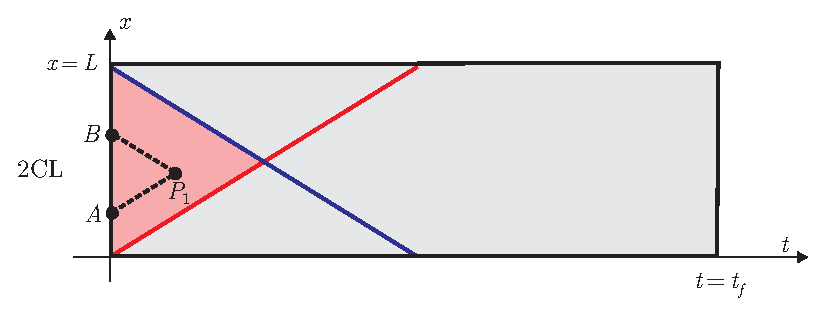
\includegraphics[width=0.8\textwidth]{mixte2a.eps} }

\bigskip

Les valeurs de $p$ et $q$ dans le triangle délimité par les caractéristiques partant des coins du domaine en $(x,t)=(0,0)$ et $(L,0)$ peuvent être calculées grâce aux caractéristiques partant de la frontière $t=0$ du domaine.


\end{slide}



%-----------------------------------------------------------------------
\begin{slide}[toc=]{Problème de Cauchy mixte - Choix des C.L.}
%-----------------------------------------------------------------------

En $P_1$, sur la frontière $x=0$, une ligne caractéristique provient de l'arc de Cauchy et ``apporte'' une relation pour calculer $p$ et $q$ (c'est une EDO ou un invariant de Riemann selon les cas). Il manque donc une seconde relation entre $p$ et $q$ pour déterminer complètement la solution.


    \centerline{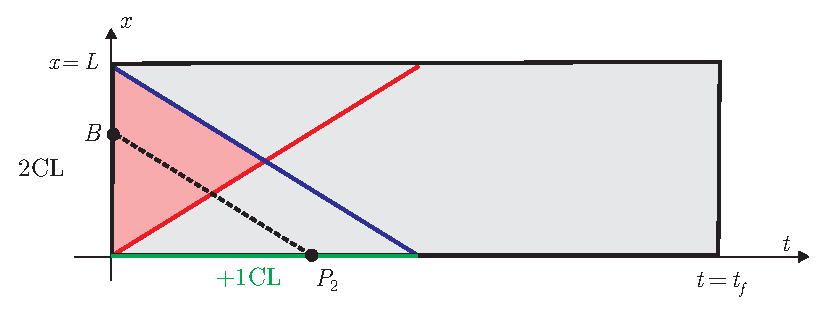
\includegraphics[width=0.8\textwidth]{mixte2b.eps} }

\bigskip

On a donc besoin d'une (et une seule) condition aux limites à cet endroit.

\end{slide}




%-----------------------------------------------------------------------
\begin{slide}[toc=]{Problème de Cauchy mixte - Choix des C.L.}
%-----------------------------------------------------------------------

De proche en proche, on constate que la solution peut être calculée dans tout le domaine si on impose une condition aux limites en $x=0$, une en $x=L$ et aucune en $t=t_f$.

\bigskip

    \centerline{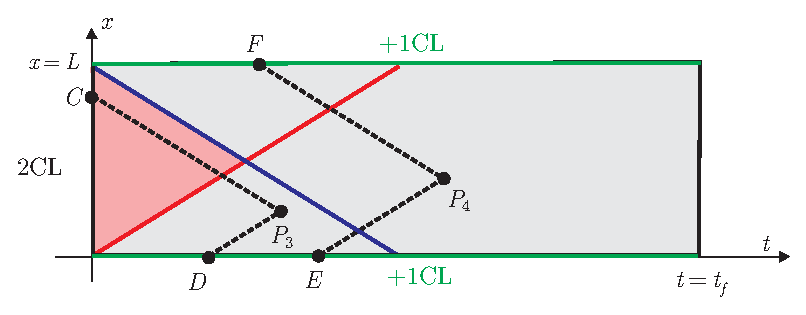
\includegraphics[width=0.8\textwidth]{mixte2c.eps} }

\bigskip

Tout comme dans le cas d'une seule équation, il peut exister plusieurs combinaisons valides de CL. Néanmoins, dans le cas où le temps est une des variables indépendantes, il est logique de choisir $t=0$ comme arc de Cauchy. On parle alors de \textbf{problème à valeurs initiales}.


\end{slide}



%-----------------------------------------------------------------------
\begin{slide}[toc=]{Problème de Cauchy mixte - Choix des C.L.}
%-----------------------------------------------------------------------

Cas plus complexe:
\bigskip

\begin{minipage}[l]{0.4\textwidth}
    \centerline{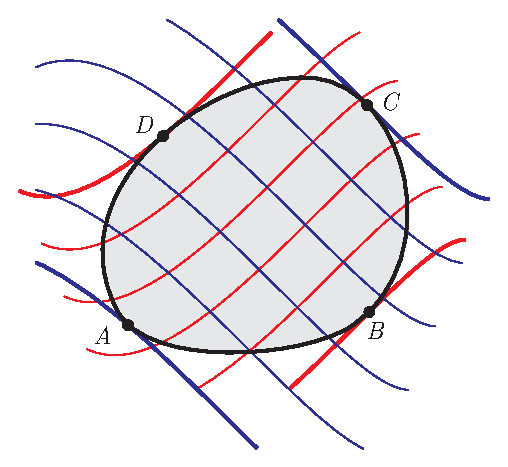
\includegraphics[width=\textwidth]{bc2a.eps} }
\end{minipage}
\begin{minipage}[l]{0.55\textwidth}
Les points de tangence des lignes caractéristiques permettent de découper la frontière du domaine étudié en plusieurs arcs ($[A,B]$, $[B,C]$, $[C,D]$ et $[D,A]$).

\bigskip

Un de ces arcs est choisi d'après la physique du problème comme arc de Cauchy sur lequel on impose le maximum de conditions (2 conditions s'il y a deux variables, comme dans cet exemple).
\end{minipage}

\bigskip

En passant d'un arc au suivant, le nombre de conditions que l'on doit imposer diminue progressivement pour atteindre un arc sur lequel on impose aucune conditions.

\end{slide}



%-----------------------------------------------------------------------
\begin{slide}[toc=]{Problème de Cauchy mixte - Choix des C.L.}
%-----------------------------------------------------------------------

Examinons deux choix possibles (parmi 4)

\bigskip

    \centerline{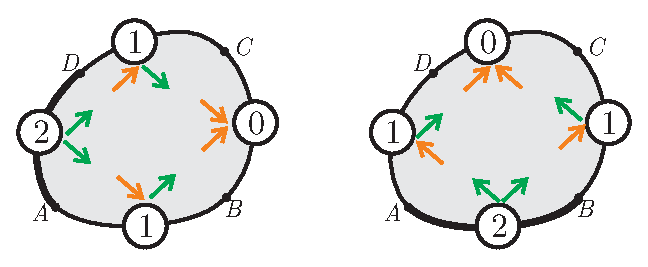
\includegraphics[width=0.7\textwidth]{bc2b.eps} }

\bigskip
\emph{Résumé de la méthode:}
\begin{itemize}
\item On choisit un arc de Cauchy.
\item On considère que les lignes quittent l'arc de Cauchy et propagent les CLs vers les autres frontières.
\item Pour chaque frontière, le nombre de CLs à imposer est égal au nombre d'inconnues moins le nombre de lignes aboutissent sur la frontière en provenance d'un autre arc.
\end{itemize}

\end{slide}


%=======================================================================
\section[toc=Carac. 3D]{Méthode des caractéristiques pour 3 variables indépendantes}
%=======================================================================

%-----------------------------------------------------------------------
\begin{slide}[toc=Extension]{Extension à plus de 2 variables indépendantes}
%-----------------------------------------------------------------------

On travaille toujours avec un système de $N$ équations du 1er ordre. Par exemple, pour 3 variables indépendantes:
\begin{equation*}
\partial_t \boldsymbol{u} + [A] \partial_x \boldsymbol{u} + \underbrace{[B] \partial_y \boldsymbol{u}}_{\text{terme suppl.}} = \boldsymbol{h}
\end{equation*}

On peut combiner les équations comme précédemment:
\begin{equation*}
\sum_{j=1}^N \left( \underbrace{a_j(\sigma_k) \partial_t + b_j(\sigma_k) \partial_x + c_j(\sigma_k) \partial_y}_{\text{dérivée directionnelle}} \right)\, u_j = \sum_{j=1}^N \sigma_j\, h_j
\end{equation*}
Néanmoins, il n'est pas possible de trouver une direction $(1,l_x,l_y)$ qui permettrait d'aligner toutes les dérivées directionnelle sur une direction unique.

\bigskip

On cherche donc plutôt l'orientation de plans dans l'espace $(t,x,y)$ orthogonaux à toutes les dérivées directionnelles précédentes. Ces plans sont les \textbf{plans caractéristiques}.

\end{slide}


%-----------------------------------------------------------------------
\begin{slide}[toc=Plans caractéristiques]{Plans caractéristiques}
%-----------------------------------------------------------------------

En un point $P$ de l'espace $(t,x,y)$ il est possible de calculer une infinité de plans caractéristiques.

    \centerline{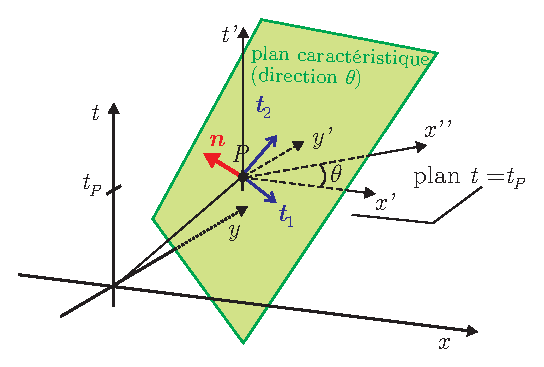
\includegraphics[width=0.6\textwidth]{plancarac.eps} }

En pratique, on travaille dans le plan $t=t_P$. Pour une direction choisie $\theta$ dans ce plan, on calcule l'inclinaison du plan caractéristique relatif à cette direction.

\end{slide}



%-----------------------------------------------------------------------
\begin{slide}[toc=]{Plans caractéristiques}
%-----------------------------------------------------------------------

Vue dans le plan $(t,x'')$ (pour un $\theta$ donné)

\bigskip

\begin{minipage}[l]{0.4\textwidth}
    \centerline{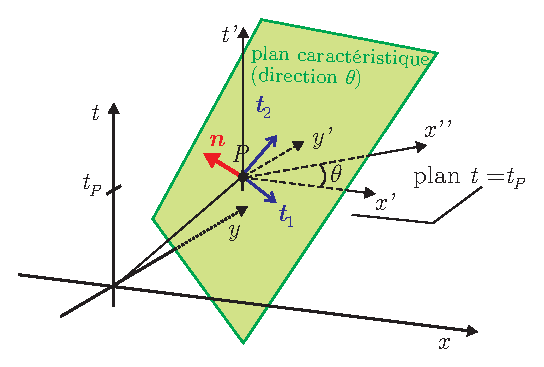
\includegraphics[width=\textwidth]{plancarac.eps} }
\end{minipage}
\begin{minipage}[l]{0.6\textwidth-1cm}
    \centerline{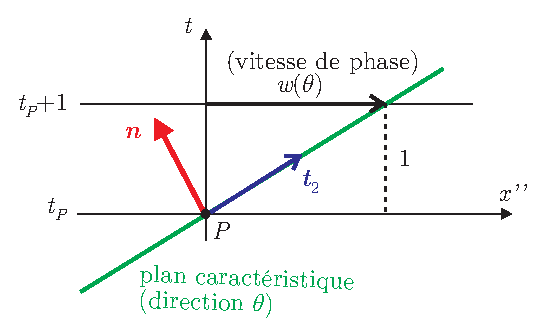
\includegraphics[width=\textwidth]{plancarac2.eps} }
\end{minipage}

\bigskip

Si la solution est telle que $\partial_{t_1} u=0$ (solution constante hors plan -- onde plane), on se retrouve dans une situation similaire à celle étudiée dans le cas de 2 variables indépendantes.

\bigskip
Le plan caractéristique décrit donc la \textbf{propagation d'une onde plane} dans la direction $\theta$.


\end{slide}




%-----------------------------------------------------------------------
\begin{slide}[toc=]{Plans caractéristiques}
%-----------------------------------------------------------------------

Vue dans le plan $(x,y)$

\bigskip

\begin{minipage}[l]{0.4\textwidth}
    \centerline{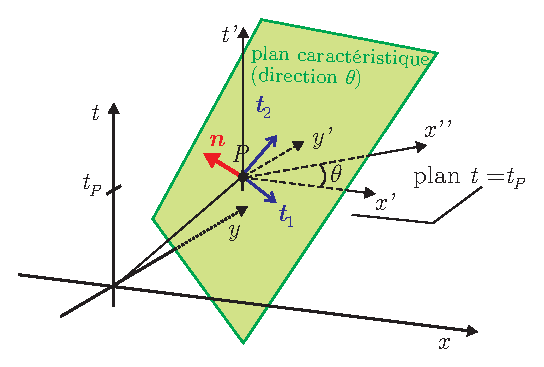
\includegraphics[width=\textwidth]{plancarac.eps} }
\end{minipage}
\begin{minipage}[l]{0.6\textwidth-1cm}
    \centerline{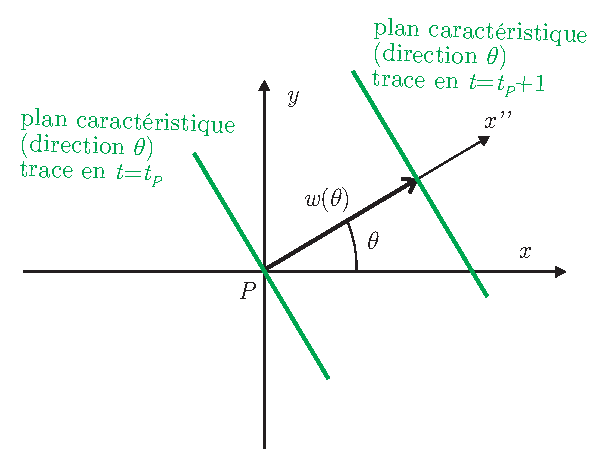
\includegraphics[width=\textwidth]{plancarac3.eps} }
\end{minipage}

\bigskip

Sur ce schéma, on a tracé l'intersection du plan caractéristique avec les plan représentant les instants $t=t_P$ et $t=t_P+1$. La distance entre ces 2 droites est la \textbf{vitesse de phase} $w$ dans la direction $\theta$.

\end{slide}


%-----------------------------------------------------------------------
\begin{slide}[toc=Vitesse de phase]{Calcul de la vitesse de phase}
%-----------------------------------------------------------------------

Exemple d'une équation d'onde simple (isotrope):
\begin{equation*}
\partial_{tt} u -a^2\partial_{xx} u -a^2\partial_{yy} u = 0
\end{equation*}

\bigskip

On étudie un mode de Fourrier:
\begin{equation*}
u(t,x,y)=U\,e^{\sigma\,t}\, e^{i\omega(\cos\theta\,x+\sin\theta\,y)}
\end{equation*}
En injectant la solution dans l'équation, on obtient:
\begin{equation*}
\sigma^2 + a^2 \omega^2 (\cos^2\theta+\sin^2\theta) = 0 \qquad \Rightarrow \quad \sigma = \pm i\,a\,\omega
\end{equation*}
La vitesse de phase s'obtient par la formule:
\begin{equation*}
w(\theta) = \frac{i\sigma}{\omega} \qquad \Rightarrow \quad \boxed{w(\theta) = \pm a }
\end{equation*}

\bigskip

Sans surprise,
\begin{itemize}
\item il y a deux familles de plans caractéristiques (puisque le système du premier ordre équivalent possède deux inconnues)
\item la vitesse de phase est indépendante de $\theta$ et vaut $+a$ pour la première famille et $-a$ pour la seconde.
\end{itemize}


\end{slide}



%-----------------------------------------------------------------------
\begin{slide}[toc=C.L.]{Conditions aux limites}
%-----------------------------------------------------------------------

Le nombre de conditions aux limites à appliquer sur une frontière du domaine de calcul est obtenu grâce à l'évaluation des vitesses de phase des différentes familles de plans caractéristiques.

    \centerline{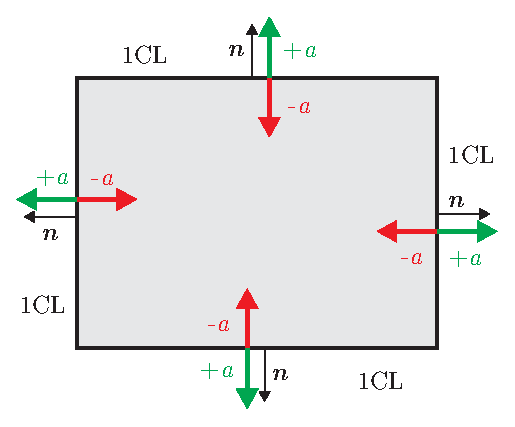
\includegraphics[width=0.5\textwidth]{bc2d.eps} }

On applique le nombre de CLs équivalent au nombre de $w$ strictement négatives selon la
normale (sortante) de la frontière concernée. En effet, toutes les vitesses positives apportent de l’info vers la frontière.


\end{slide}




\end{document}




